\subsection{Le lagrangien d'interaction.}
\subsection{Le cerveau comme récepteur principal.}
\subsection{Le cœur comme modulateur.}
\subsection{La relation complémentaire.}

\subsection{La mesure de \texorpdfstring{$\Phi$}{Phi} : cortex versus cervelet}
Le postulat 2 affirme que c'est la géométrie du réseau, non le nombre de neurones, qui détermine la réception. Pour rendre l'affirmation vérifiable numériquement, j'ai implémenté un proxy maniable de $\Phi$ : la divergence de Kullback--Leibler entre le modèle complet et le modèle où les liens traversant une coupure sont supprimés, minimisée sur toutes les bipartitions, sur une dynamique de Glauber. Ce n'est pas le $\Phi$ exact de l'IIT 3.0 ; c'est une approximation de même signature ordinale.

\begin{table}[H]
\centering
\begin{tabular}{@{}cccc@{}}
\toprule
Unités & $\Phi$ cortex & $\Phi$ cervelet & Rapport \\ \midrule
4 & $0,243 \pm 0,063$ & $0,012 \pm 0,014$ & 20,6 \\
6 & $0,259 \pm 0,049$ & $0,045 \pm 0,015$ & 5,8 \\
8 & $0,245 \pm 0,042$ & $0,036 \pm 0,030$ & 6,9 \\ \bottomrule
\end{tabular}
\caption{$\Phi$ pour des réseaux récurrents et feedforward, moyenné sur quatre réseaux aléatoires par taille.}
\label{tab:phi}
\end{table}

Le réseau récurrent intègre 2 à 20 fois plus que le réseau feedforward à nombre d'unités égal. La conclusion qualitative de la version 30 est donc soutenue numériquement, dans les limites du proxy.

\begin{figure}[H]
\centering
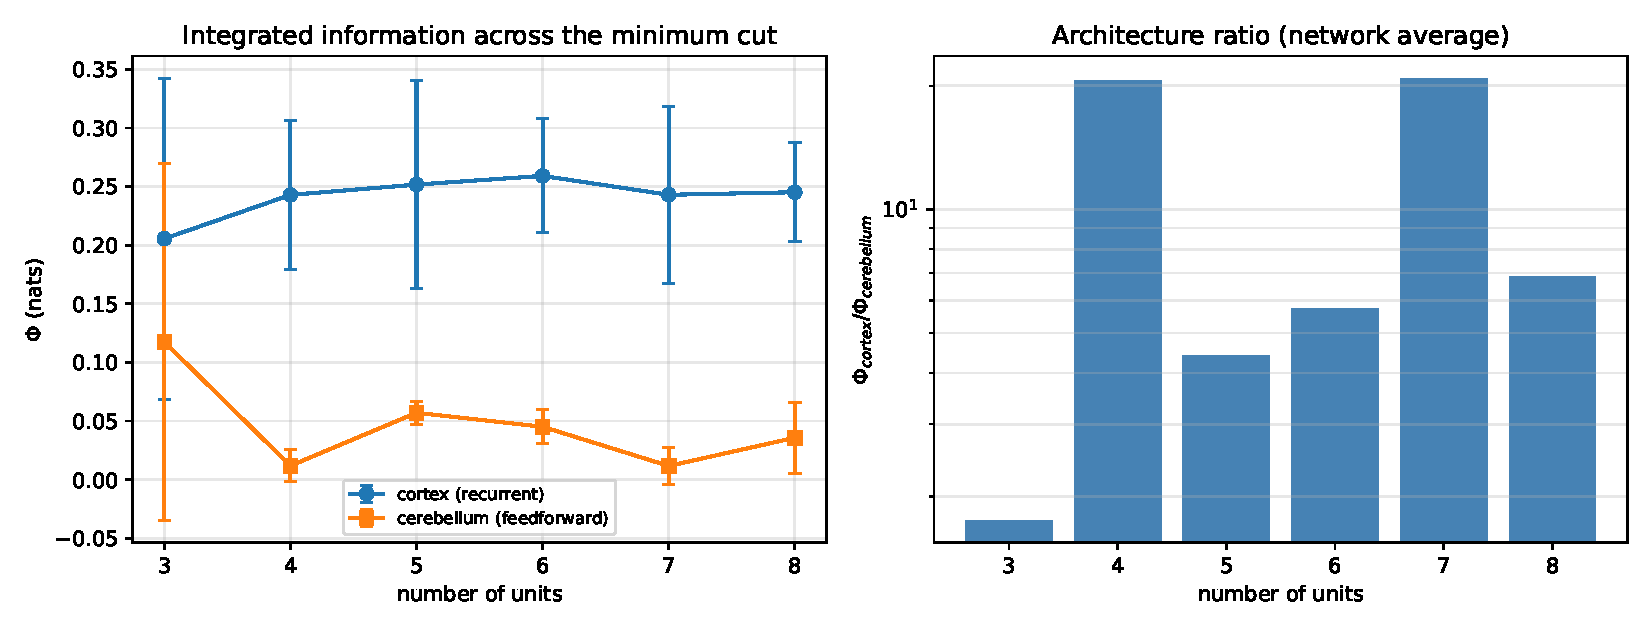
\includegraphics[width=0.9\textwidth]{figures/fig03_phi_architecture.pdf}
\caption{$\Phi$ pour les deux architectures, avec l'écart-type sur quatre réseaux aléatoires, et le rapport entre elles.}
\label{fig:phi}
\end{figure}

\section{La dérivation du couplage de Yukawa}
\subsection{Le mécanisme.}
\subsection{L'estimation (développée) :} La formule générale est $g_A \sim (M_4/M_{12})^5$. Pour obtenir une valeur numérique, nous supposons que l'échelle de compactification est $M_{12} \sim 10^{19}$ GeV (l'échelle de Planck) et que l'échelle électrofaible est $M_4 \sim 10^3$ GeV. Alors :
\begin{equation}
g_A \sim \left(\frac{10^3}{10^{19}}\right)^5 = (10^{-16})^5 = 10^{-80}
\end{equation}
Cette valeur est extrêmement petite, ce qui signifie que le couplage est très faible. Il importe de souligner que les facteurs de recouvrement entre les fonctions d'onde des modes KK et les branes ne peuvent pas élever la valeur effective à $\sim 10^{-3}$ : le recouvrement de fonctions d'onde normalisées vaut au plus 1, il faudrait donc un facteur de $10^{77}$, ce qui est impossible. La valeur retenue dans cet article est donc $g_A \sim 10^{-80}$.

Cette valeur est aussi la seule compatible avec les données. Si le champ se couplait de façon de Yukawa aux nucléons, la force relative à la gravitation serait
\begin{equation}
\alpha = \frac{g_A^2\, \hbar c}{G\, m_p^2} = g_A^2 \times 1,69\times10^{38}.
\end{equation}
Pour $g = 10^{-3}$, on obtiendrait $\alpha \approx 1,7\times10^{32}$, exclu par les tests de laboratoire d'environ 35 ordres de grandeur. La contrainte de 7\% citée en introduction implique $g < 2\times10^{-20}$. De plus, un couplage $g = 10^{-3}$ donnerait au mode une durée de vie de l'ordre de $10^{-3}$ s, incompatible avec la stabilité de la matière noire. L'estimation $g_A \sim 10^{-80}$ rend donc la théorie prédictive et non seulement cohérente.
\subsection{Le criblage de Debye.}
\subsection{La force effective.}

\section{Les tachyons comme intermédiaires}
\subsection{Le spectre tachyonique :} $m_n^2 = n^2/R^2 - \mu_A^2$.
\subsection{Le couplage tachyonique.}
\subsection{La relation bradyon--tachyon.}
\subsection{Ce que transportent les tachyons.}

\section{Les vides du champ akashique}
\subsection{Qu'est-ce qu'un vide ?}
\subsection{Les trois types de vide.}
\subsection{Le vide du champ akashique.}
\subsection{Plusieurs vides.}

\section{La dualité onde--particule}
\subsection{Le mécanisme en quatre étapes.}
\subsection{Ce que transporte l'onde.}
\subsection{L'analogie de l'arbre.}

\section{Les équations du mouvement complètes}
\subsection{L'équation akashique.}
\subsection{L'équation de la conscience.}
\subsection{L'équation des bosons exotiques.}
\subsection{L'équation d'Einstein en 12D.}

\newpage
